\section{Vooronderzoek}

\subsection{Neuraal netwerk}
Neurale netwerken zijn een reeks algoritmen die losjes gemodelleerd zijn van het menselijke brein. Een artificial brein dat gemaakt is uit een hele grote reeks artificial neurons.
%Wat is artificial? Goed om uit te leggen en in woordenlijst te douwen :)

\subsubsection{Perceptrons}
Een van de meest fundamenteele artifical neuron types is een perceptron. Perceptronen zijn een belangrijk onderdeel van een neuraal netwerk en kennis hierover is nodig om een neuraal netwerk te begrijpen. Een perceptron pakt verschillende binary inputs:$x_{1}, x_{2},....x_{n}$ en produceerd een enkele binaire output. Je kan het zien als een functie die beslissingen voor je neemt, door verschillende factoren tegen elkaar te wegen en uiteindelijk met ja of nee te antwoorden.
\begin{figure}[h!]
\centering
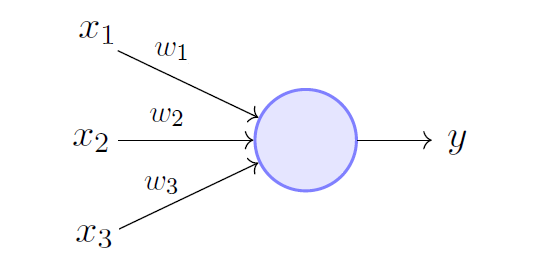
\includegraphics[scale=0.5]{perceptron2.png}
\caption{uitleg}
\label{peceptron2}
\end{figure}
\linebreak
In afbeelding \ref{peceptron2} is een perceptron te zien die 3 variabelen als input neemt: $x_{1}, x_{2}$ en $x_{3}.$ Bij all deze waardes word een gewicht(weight) toegekend($w_{n}$). Deze waarde geeft aan hoe belangrijk de input is voor deze neuron. De output van de neuron is de som van alle resultaten bij elkaar. $\sum_{j}w_{j}x_{j}$ en deze waarde vergelijken met een gekozen randwaarde(threshold) om de output the berekenen. In een meer wiskundige term:
%\begin{equation*} %tTODO write function
%\begin{rcases}
%        0  if \sum_{j}w_{j}x_{j}+b $\leq$ threshold $\\$
%        1  if \sum_{j}w_{j}x_{j}+b > threshold
%\end{rcases} 
%$\text{output}$
%\end{equation*}
 \begin{equation}
    y(x_1,\ldots,x_n) = f(w_1x_1 + w_2x_2 + \ldots + w_nx_n)  \label{per-eq}
  \end{equation}

\noindent Je kan de output van een neuron beinvloeden door te spelen met de weights en thresholds. Door een input zijn weight te vergroten of de threshold te verlagen kan er hele andere resultaten uit het model komen.\\
\newline
Het is duidelijk dat de perceptron niet een compleet model is over hoe mensen hun beslissingen nemen. Maar het voorbeeld illustreert hoe een perceptron verschillende soorten bewijs kan afwegen om beslissingen te nemen. Daarom is het aannemelijk dat een complex netwerk van perceptrons vrij subtiele beslissingen zou moeten kunnen nemen.
\begin{figure}[h!]
\centering
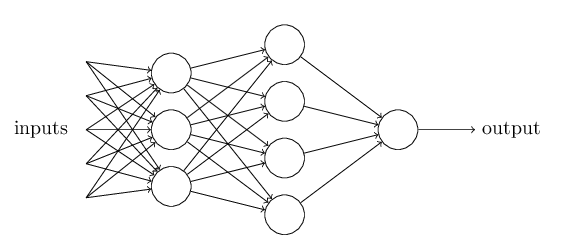
\includegraphics[scale=0.5]{perceptron3.png}
\caption{uitleg}
\label{perceptron3}
\end{figure}
\newline
In afbeelding \ref{perceptron3} is een netwerk te zien, waar de eerste laag van perceptrons in het netwerk, drie simpele beslissingen neemt door de functie in vergelijking \ref{per-eq} uit te voeren. Naast de eerste laag zit er nu ook een tweede die de outputs van de eerste laag als input neemt. Op deze manier kan een perceptron in de tweede laag een beslissing nemen op een complexer en abstracter niveau dan perceptrons in de eerste laag. Deze complexiteit en abstractheid word verhoogd per extra laag dat je toevoegd. Op deze manier kan een meerlaags netwerk van perceptrons, zeer geavanceerde beslissingen nemen.\\
\newline
De volgende stap is om ons netwerk zelf lerend te maken. Om dit te doen moet je kleine aanpassingen kunnen maken aand de weights en de biases. Deze kleine aanpassingen moet daarna ook een klein effect hebben op de output van het neurale netwerk. Echter dat is niet wat er gebeurt met perceptronen want deze heeft maar 2 outputs, een 1 en een 0. Een kleine aanpassing zal daarom niks doen of de hele uitkomst van de perceptron omdraaien. Je kan niet probleem omzeilen door een ander types neurons te gebruiken ,zoals de Sigmoid en tanh neurons.

\subsubsection{tanh neurons}
sigmoid en tanh neurons lijken erg op perceptrons alleen de manier hoe de ouput berekend word is anders. 


\subsection{python}

\subsection{Encog}